% -----------------------------------------------------------------
% Document class: Article
\documentclass[ a4paper, twoside, 11pt]{article}
\usepackage{../../macros-general}
\usepackage{../../macros-article}
% Number of the handout, quiz, exam, etc.
\newcommand{\numero}{03}
\setcounter{numero}{\numero}

% -----------------------------------------------------------------
\begin{document}
\allowdisplaybreaks

% Indices
\newcommand{\iava}{$i$\tsup{ava} }
\newcommand{\iavo}{$i$\tsup{avo} }
\newcommand{\java}{$j$\tsup{ava} }
\newcommand{\javo}{$j$\tsup{avo} }
\newcommand{\kava}{$k$\tsup{ava} }
\newcommand{\kavo}{$k$\tsup{avo} }
\newcommand{\tava}{$t$\tsup{ava} }
\newcommand{\tavo}{$t$\tsup{avo} }
\newcommand{\tmava}{$(t-1)$\tsup{ava} }
\newcommand{\tmavo}{$(t-1)$\tsup{avo} }
\newcommand{\tMava}{$(t+1)$\tsup{ava} }
\newcommand{\tMavo}{$(t+1)$\tsup{avo} }

\begin{center}
\Large Modelos Estoc\'asticos (INDG-1008): Lecci\'on \numero \\[1ex]
\small \textbf{Semestre:} 2018-2019 T\'ermino I \qquad
\textbf{Instructor:} Luis I. Reyes Castro
\end{center}
\fullskip

% -----------------------------------------------------------------
\begin{problem}
En un call center se atienden a dos tipos de clientes desde las 9:00 AM. \linebreak Las llamadas de los clientes tipo 1 y tipo 2 constituyen procesos Poisson independientes con media de 4.2 y 6.5 minutos, respectivamente. 
\begin{enumerate}[label=\textbf{\alph*)}]
\item \textbf{[2 Puntos]} Si se recibe una llamada de un cliente tipo 1 a las 9:04 AM, cu\'al es el tiempo esperado hasta la primera llamada de un cliente tipo 2?
\item \textbf{[2 Puntos]} Si nadie ha llamado hasta las 9:07, cu\'al es la probabilidad de que la primera llamada llegue antes de las 9:12?
\end{enumerate}

\end{problem}
\fullskip

% -----------------------------------------------------------------
\begin{problem}
\textbf{[4 Puntos]} Encuentre la pol\'itica \'optima para el siguiente \'arbol de decisi\'on. 

\begin{figure}[htb]
\centering
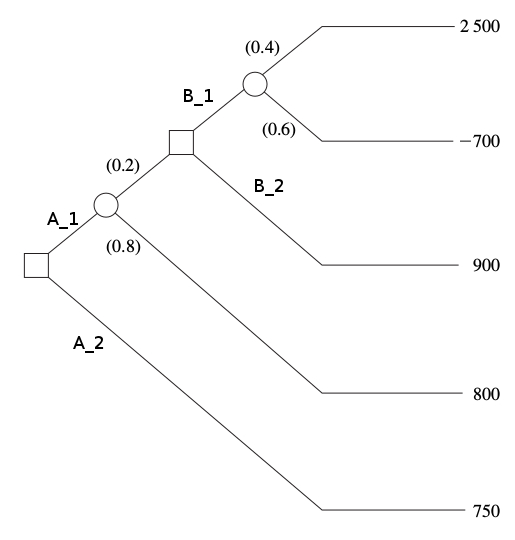
\includegraphics[width=0.6\columnwidth]{problema_arbol-decision.jpg}
\end{figure}

\end{problem}
\fullskip

% -----------------------------------------------------------------
\begin{problem}
\textbf{[8 Puntos]} Como parte de las preparaciones para la Liberaci\'on de Venezuela, la Agencia Central de Inteligencia de EE.UU. (CIA, por sus siglas en ingl\'es) ha contratado al malvado e inescrupuloso Prof. Reyes para escribir un virus de computadora capaz de desahibilitar sistemas de radar de origen ruso o sovi\'etico. Con este prop\'osito, el profesor ha desarrollado un virus estoc\'astico con una memoria de tres pasos capaz de re-escribir al azar los bits de memorias electr\'onicas. El virus funciona de la siguiente manera: 
\begin{enumerate}
\item Se empieza con una secuencia de tres d\'igitos, cada uno de los cuales puede tomar los valores cero o uno al azar con probabilidad uniforme. 
\item En cada paso, se escoge el siguiente d\'igito al azar pero en funci\'on de los tres d\'igitos anteriores. En particular, sup\'ongase que de los tres d\'igitos anteriores $k$ de ellos son unos. Entonces: 

\begin{table}[H]
\centering
\begin{tabular}{|c|c|}
\hline
$\boldsymbol{k}$ & $\Pr$( siguiente d\'igito = 1 ) \\ \hline
0 & 0.20 \\ \hline
1 & 0.40 \\ \hline
2 & 0.60 \\ \hline
3 & 0.80 \\ \hline
\end{tabular}
\end{table}

\end{enumerate}

Con esto en mente, modele el comportamiento de este virus como una Cadena de Markov. \\[1ex] \emph{Sugerencia:} Recuerde que los modelos de Cadenas de Markov tienen memoria de un solo paso. Por lo tanto, usted querr\'a modelar el virus como una cadena con un estado para cada posible combinaci\'on de los tres d\'igitos.

\QED

\end{problem}
\fullskip

\end{document}
